\section{Harmonic and melodic minor scale}

The minor scale that you have seen no far is also called the 'natural' minor scale. The harmonic and melodic minor scales are alternations on this.

This section assumes that you have already read \autoref{sec:minor_scale} or know about the natural minor scale.

\subsection{Harmonic minor}

The harmonic minor scale is the same as the natural minor scale, but is has a raised 7th degree. See \autoref{tab:guitar_harmonic_minor_scale_interval}. The \textbf{W+} here means 3 half steps, or 1,5 whole steps.

\begin{table}[h]
	\centering
	\begin{NiceTabular}{*{16}{P{0.05mm}}}
		\Block{}{} & \Block{1-2}{\large{W}} & & \Block{1-2}{\large{H}} & & \Block{1-2}{\large{W}} & & \Block{1-2}{\large{W}} & & \Block{1-2}{\large{H}} & & \Block{1-2}{\large{W+}} & & \Block{1-2}{\large{H}} & & \Block{}{} \\
		\Block{1-2}{1} & & \Block{1-2}{2} & & \Block{1-2}{3$\flat$} & & \Block{1-2}{4} & & \Block{1-2}{5} & & \Block{1-2}{6$\flat$} & & \Block{1-2}{7} & & \Block{1-2}{8} & 
	\end{NiceTabular}
	\caption{Harmonic Minor scale intervals}
	\label{tab:guitar_harmonic_minor_scale_interval}
\end{table}

To create, for example, the C minor scale we will start on the C and then simply follow the formula. One possible way to play it is shown in \autoref{fig:guitar_c_harmonic_minor_scale_first_position}.

\begin{table}[h]
	\centering
	\begin{NiceTabular}{*{16}{P{0.05mm}}}
		\Block{}{} & \Block{1-2}{\large{W}} & & \Block{1-2}{\large{H}} & & \Block{1-2}{\large{W}} & & \Block{1-2}{\large{W}} & & \Block{1-2}{\large{H}} & & \Block{1-2}{\large{W+}} & & \Block{1-2}{\large{H}} & & \Block{}{} \\
		\Block{1-2}{1} & & \Block{1-2}{2} & & \Block{1-2}{3$\flat$} & & \Block{1-2}{4} & & \Block{1-2}{5} & & \Block{1-2}{6$\flat$} & & \Block{1-2}{7} & & \Block{1-2}{8} & \\
		\Block{1-2}{C} & & \Block{1-2}{D} & & \Block{1-2}{E\flat} & & \Block{1-2}{F} & & \Block{1-2}{G} & & \Block{1-2}{A\flat} & & \Block{1-2}{B} & & \Block{1-2}{C} & 
	\end{NiceTabular}
	\caption{C harmonic minor scale}
	\label{tab:guitar_c_harmonic_minor_scale}
\end{table}


\begin{figure}[h]
	\centering
	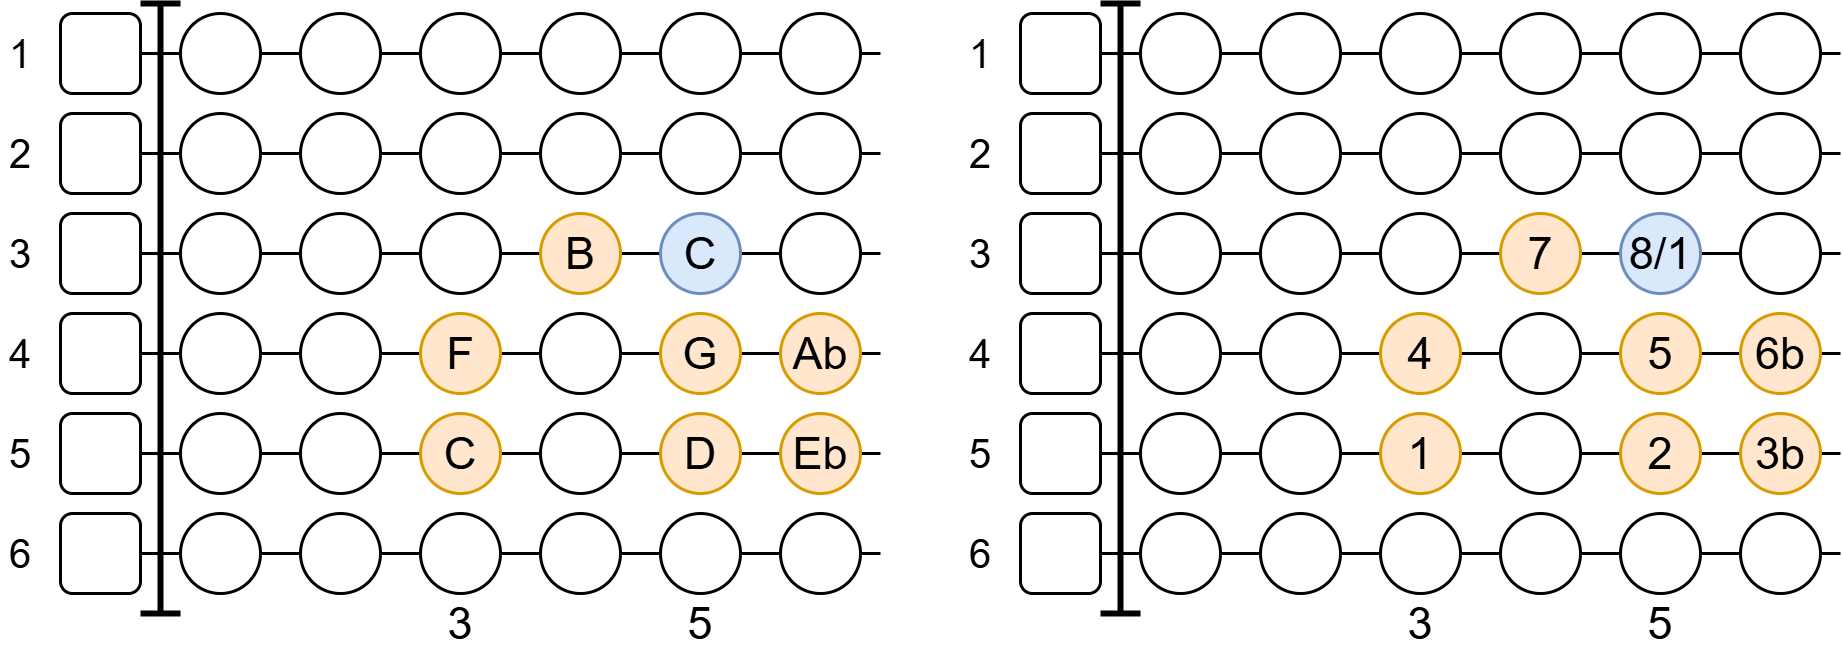
\includegraphics[height=0.2\textheight]{../../Images/CHarmonicMinorScaleFirstPosition.png}
	\caption{C harmonic minor scale described with note names and with intervals}
	\label{fig:guitar_c_harmonic_minor_scale_first_position}
\end{figure}

\newpage

\subsubsection{Getting a feeling for the harmonic minor scale}

A way to get a good feeling for what the minor scale would 'feel' is to play the root of the harmonic minor scale as a drone note and then playing the notes from the harmonic minor scale on a single string over it. Taking the E harmonic minor scale as an example (\autoref{fig:harmonic_minor_scale_with_drone_single_string}). Play the open low E string and play a melody on the 4th string using the harmonic minor scale. You will hear which interval gives what type of relation to the root.

\begin{figure}[h]
	\centering
	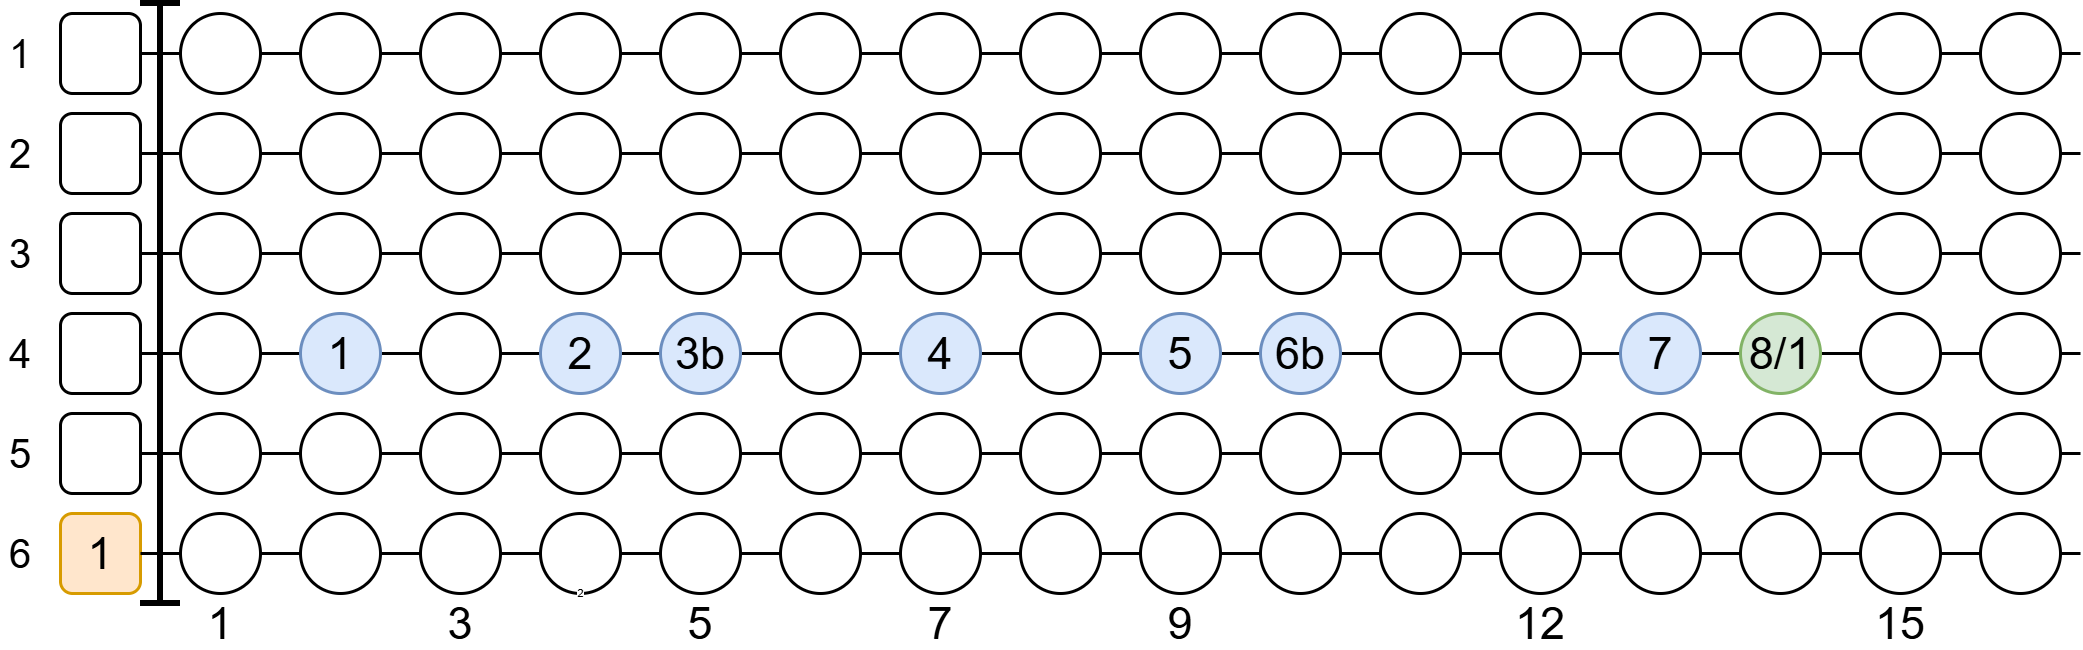
\includegraphics[height=0.18\textheight]{../../Images/harmonic_minor_scale_drone_single_string.png}
	\caption{E harmonic minor on a single string with an open E string drone}
	\label{fig:harmonic_minor_scale_with_drone_single_string}
\end{figure}

\subsection{Melodic minor}
TODO

% \section{Blues scale}